\subsection{Electron Channel Selection}
\label{sec:electronId}


Electrons are identified offline as clusters of ECAL energy deposits
matched to tracks reconstructed in the silicon tracker.
The ECAL clustering algorithm is designed to reconstruct clusters containing a
large fraction of the energy of the original electron, including energy
radiated along its trajectory. The ECAL clusters must fall in the ECAL fiducial volume
of $|\eta| < 1.44$ for EB clusters or $1.57 < |\eta| < 2.5$ for EE clusters.
The transition region $1.44 < |\eta| < 1.57$ is excluded as it leads to lower-quality
reconstructed clusters, due mainly to services and cables exiting between the barrel and
endcap calorimeters. Electron tracks are reconstructed using an algorithm~\cite{GSF} 
(Gaussian-sum filter, or GSF tracking) that accounts for possible energy loss due to 
bremsstrahlung in the tracker layers. 


%%%%%
\begin{figure}[htbp]
  \begin{center}
   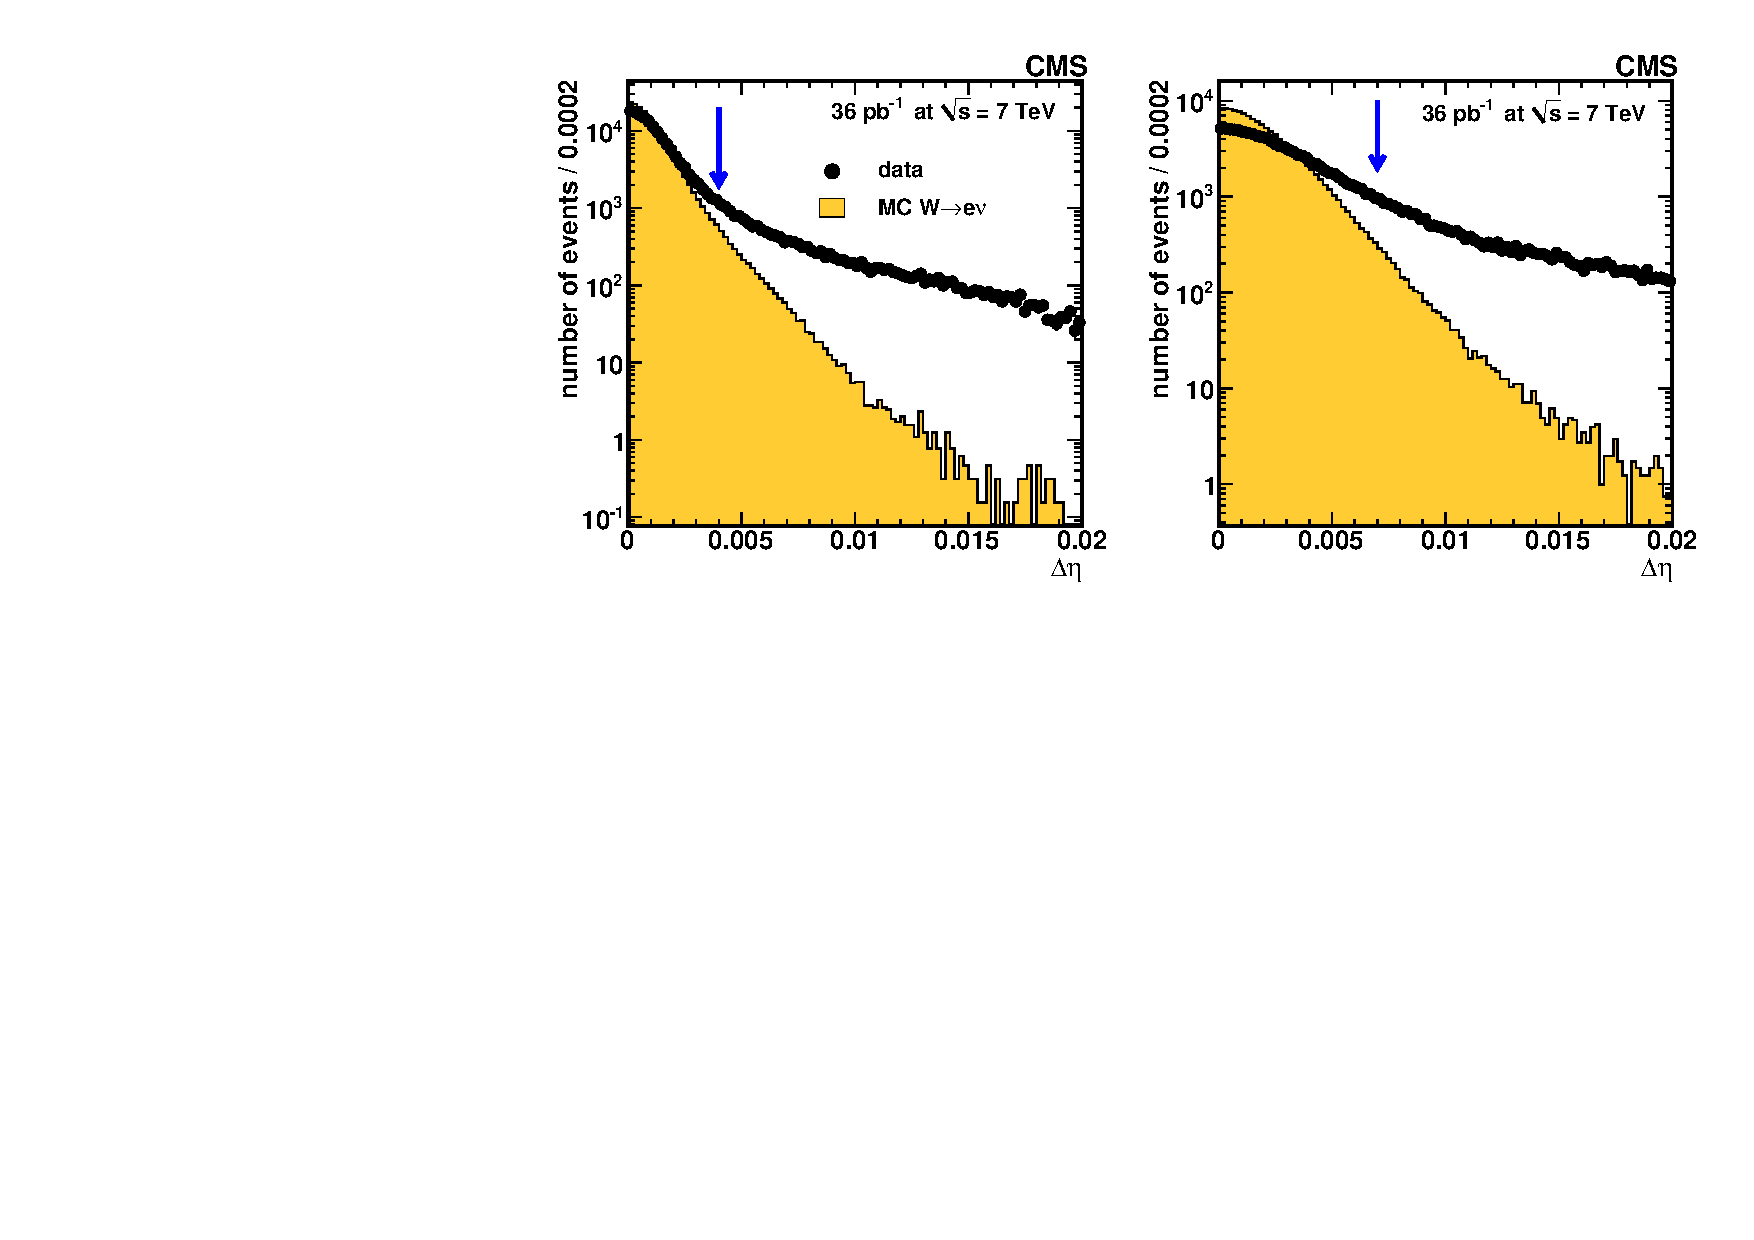
\includegraphics[width=0.68\textwidth]{figs/deta.pdf}
   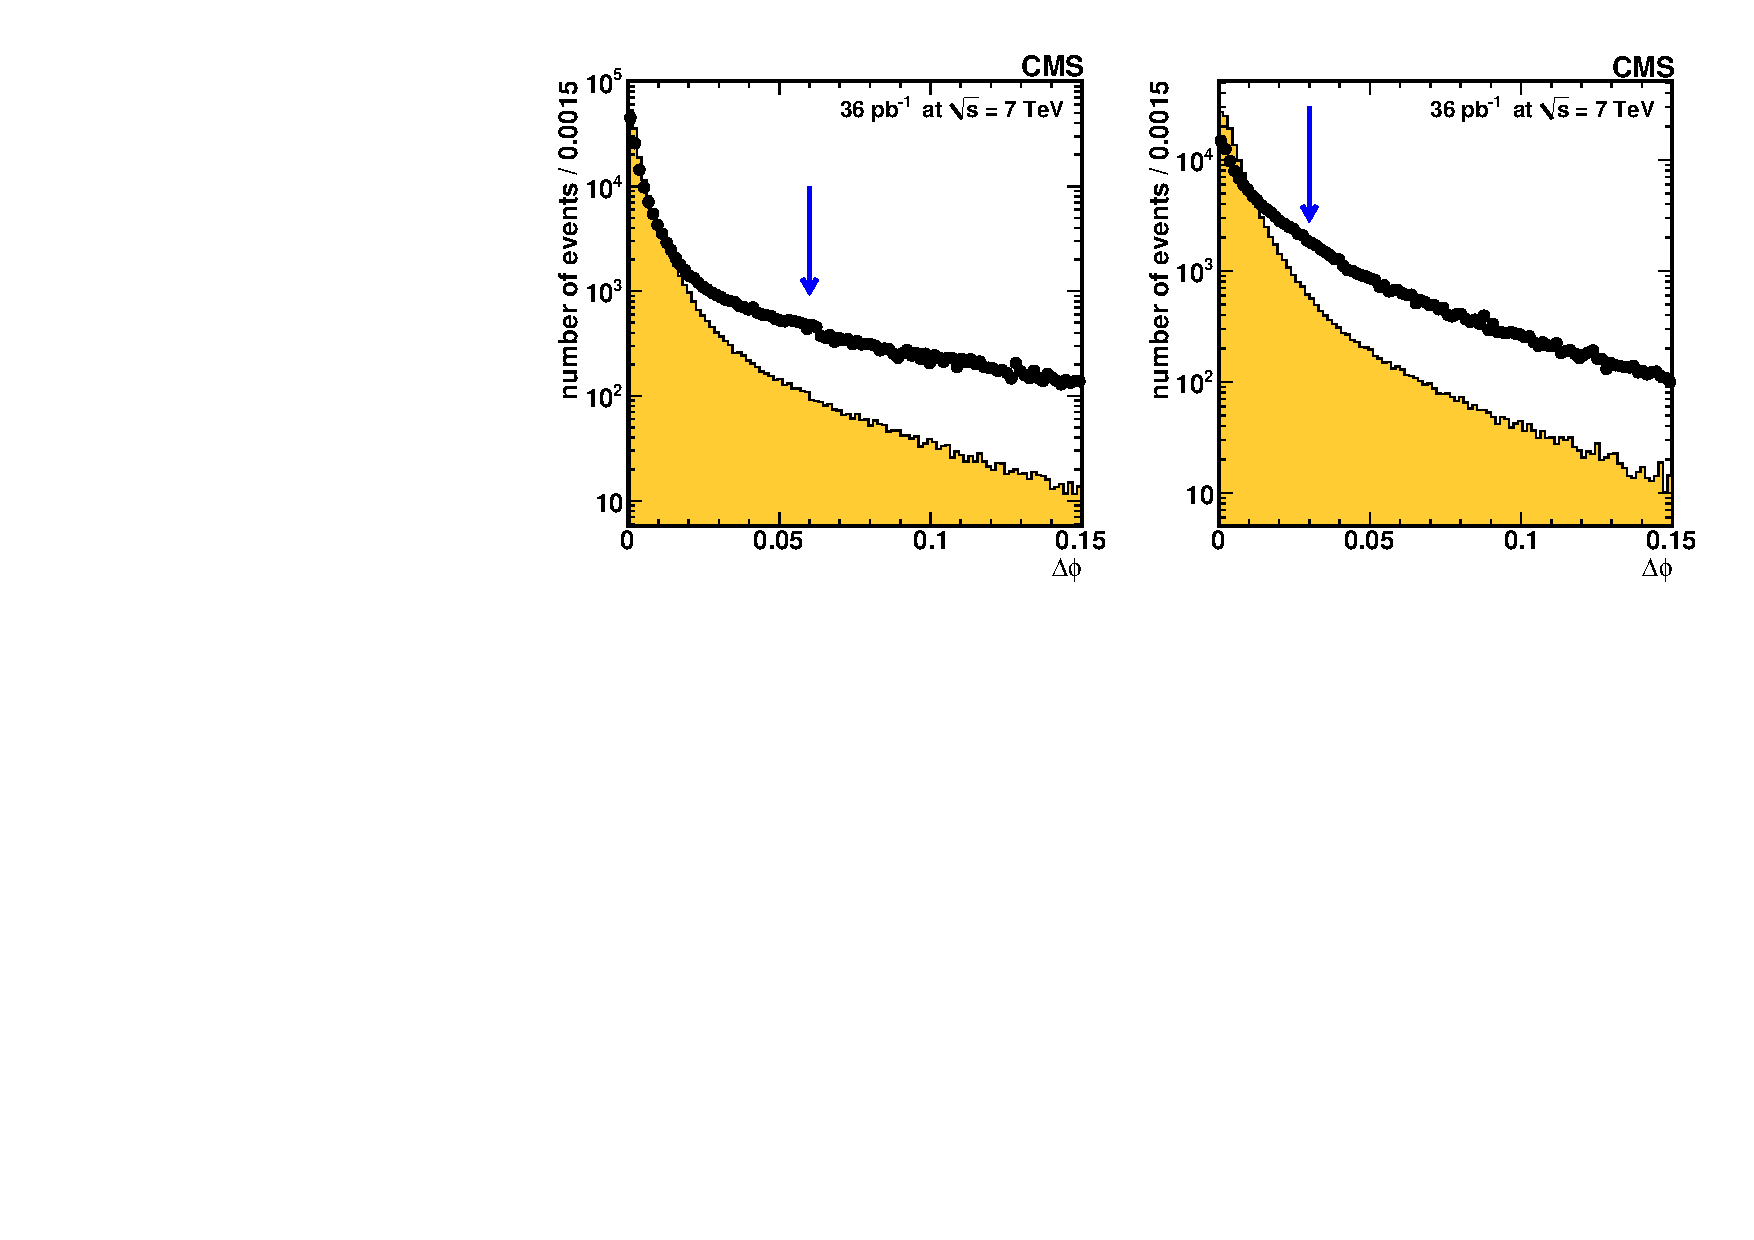
\includegraphics[width=0.68\textwidth]{figs/dphi.pdf}
   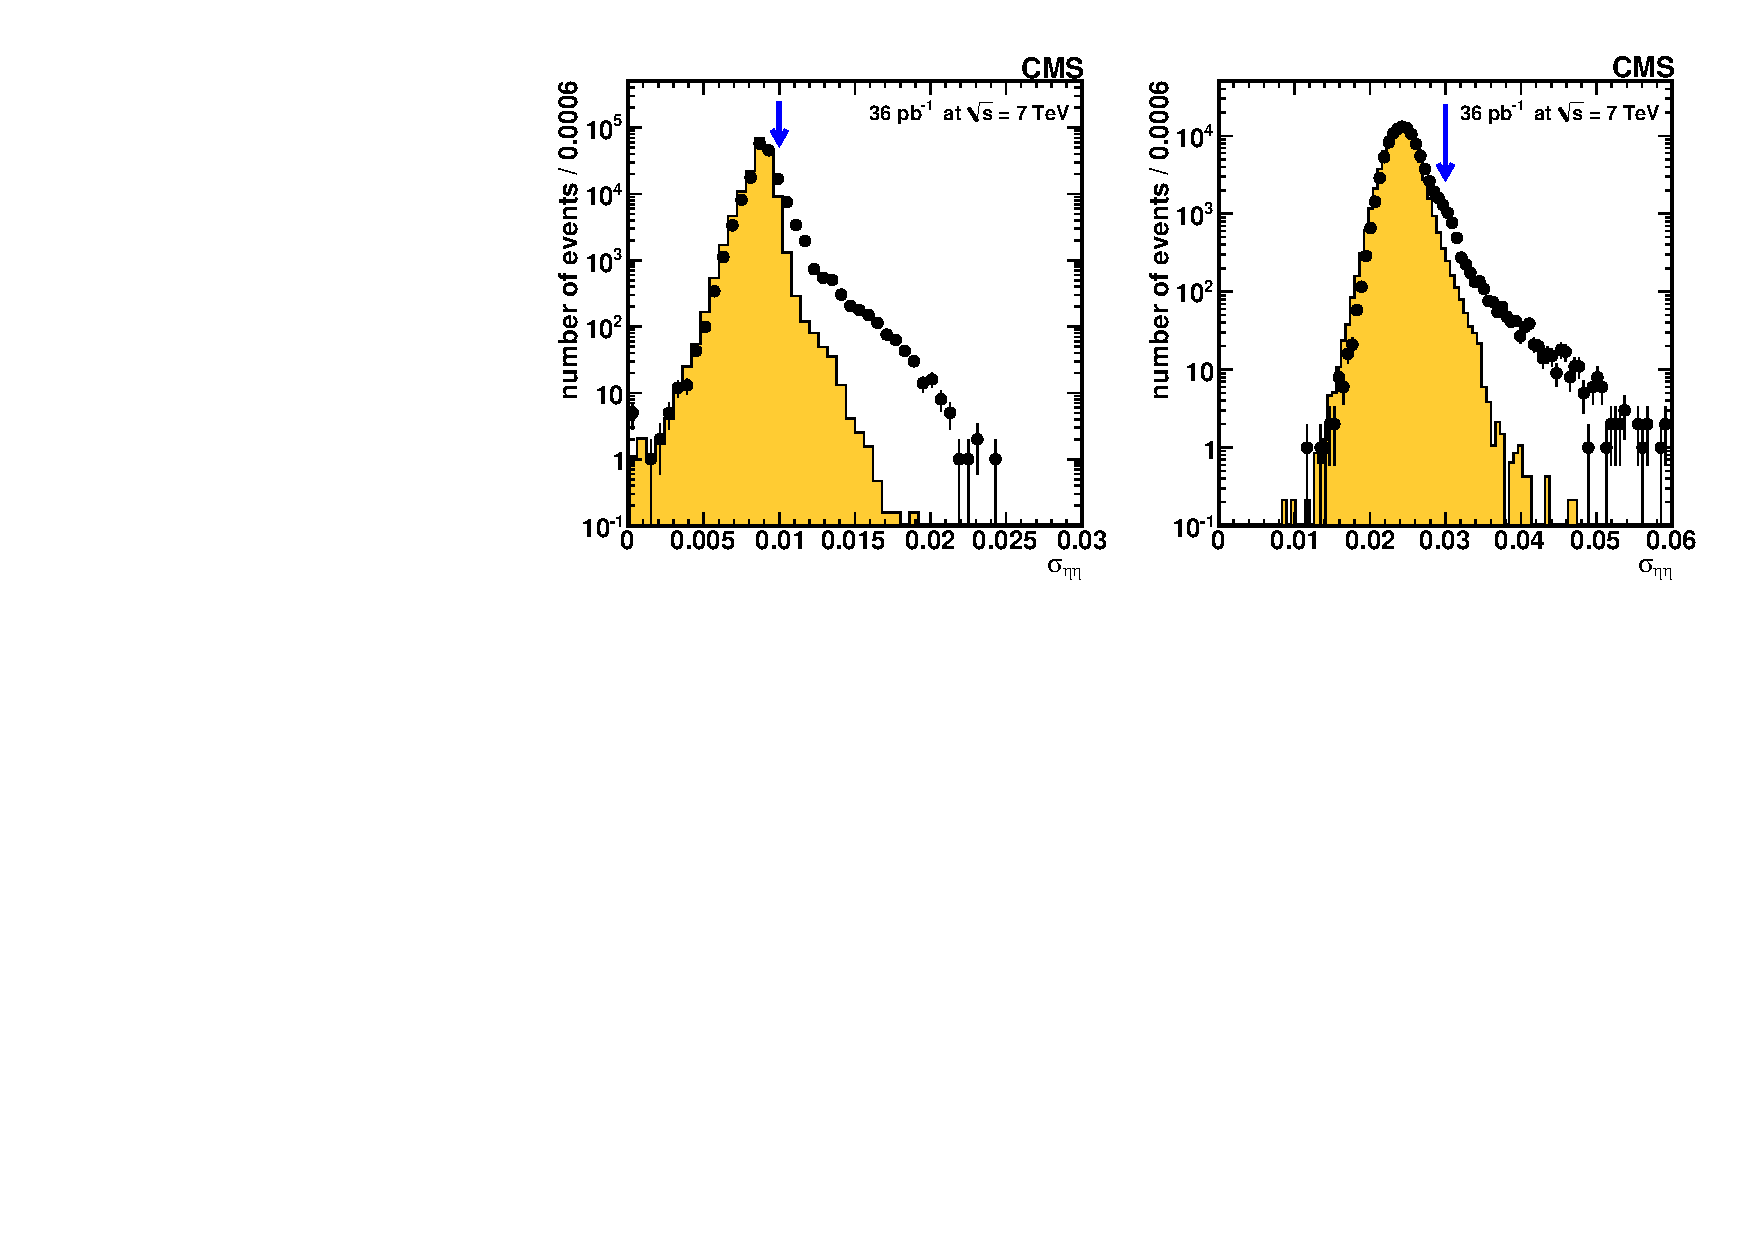
\includegraphics[width=0.68\textwidth]{figs/sihih.pdf}
   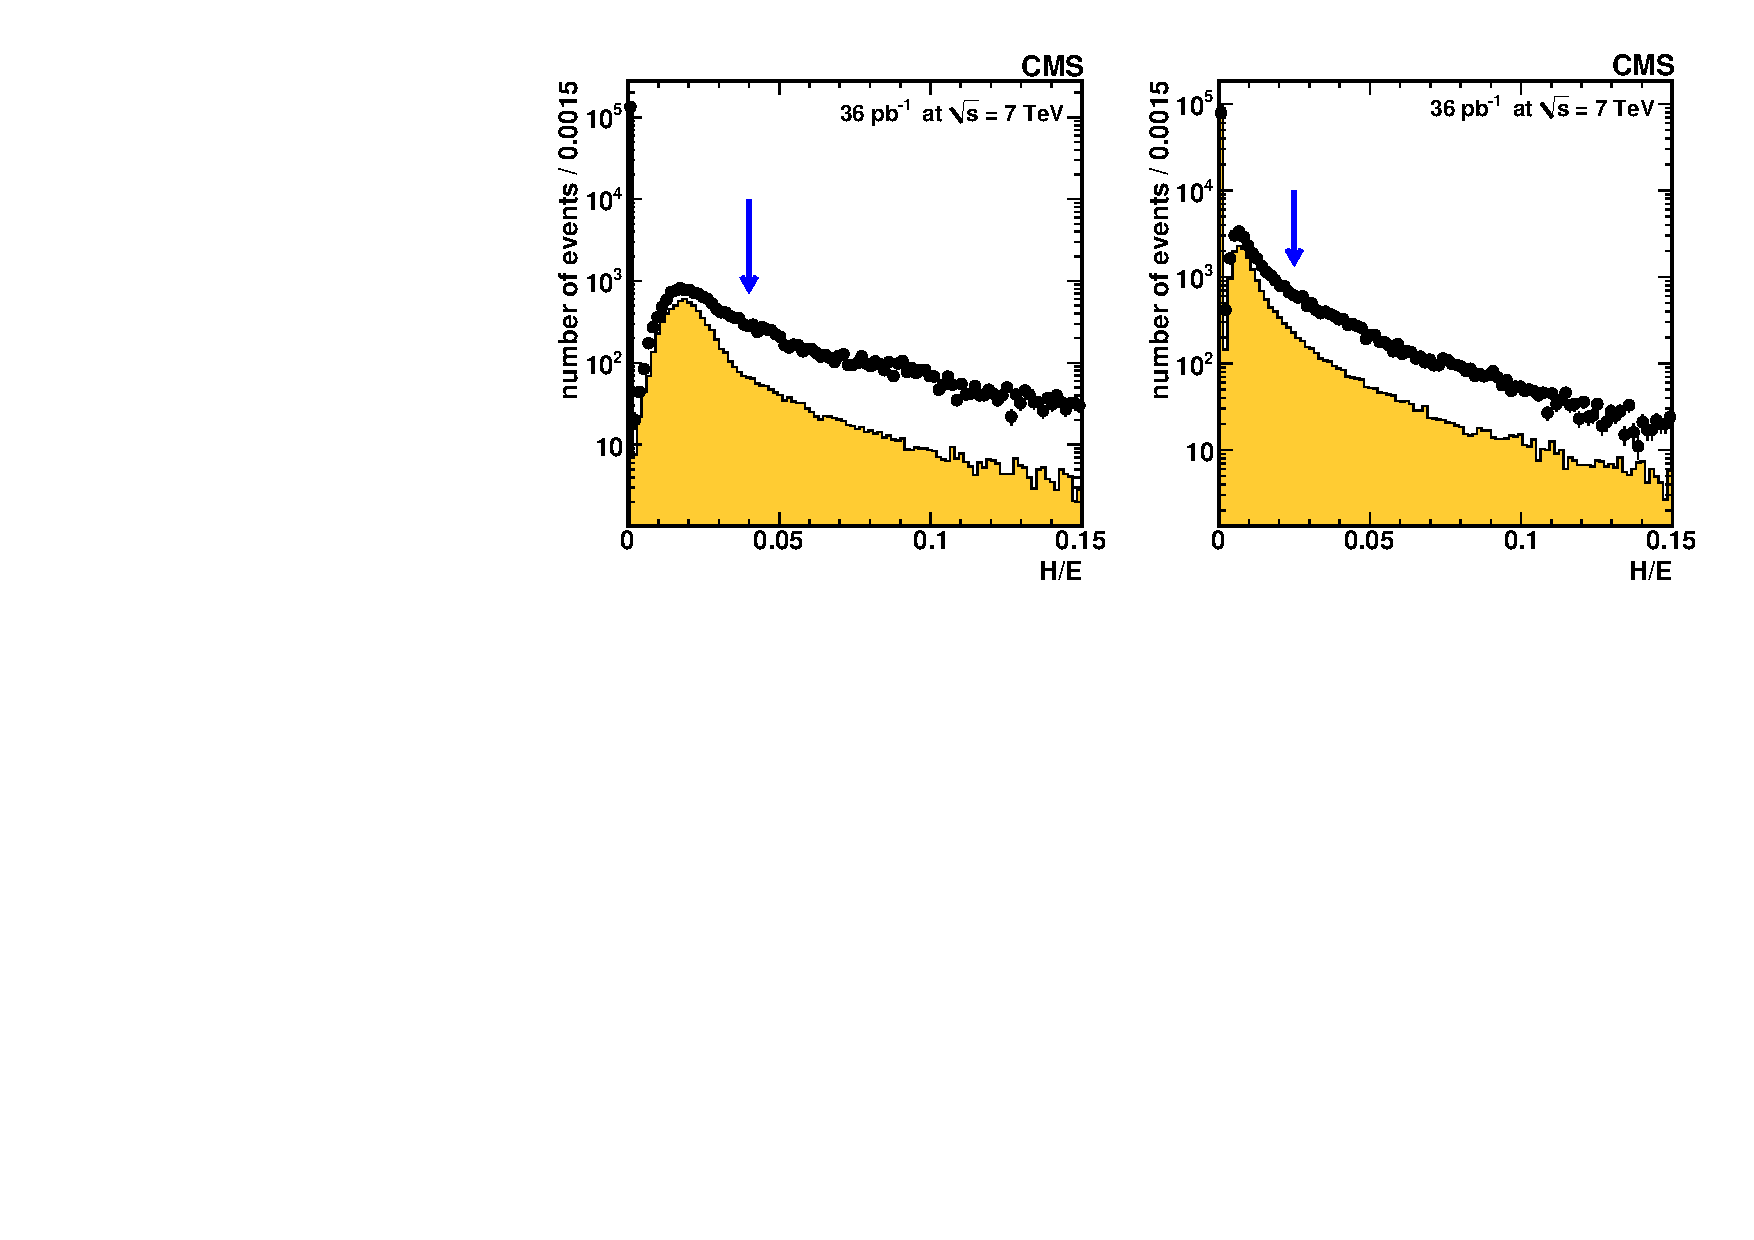
\includegraphics[width=0.68\textwidth]{figs/hoe.pdf}
   \caption{ \label{fig:WenuSelection1}
Distributions of the electron identification variables $\Delta\eta$, $\Delta\phi$, $\sigma_{\eta\eta}$, 
and $H/E$ for data (points with the error bars), for EB (left) and EE (right).
For illustration the simulated $\Wen$ signal (histograms), normalized to the number of events
observed in data, is superimposed.
These distributions are obtained after applying all 
the tight requirements on the selection variables, except that on the presented
variable. The tight requirement on that variable is indicated with an arrow. }
  \end{center}
\end{figure}
%%%%%

%%%%%
\begin{figure}[htbp]
  \begin{center}
   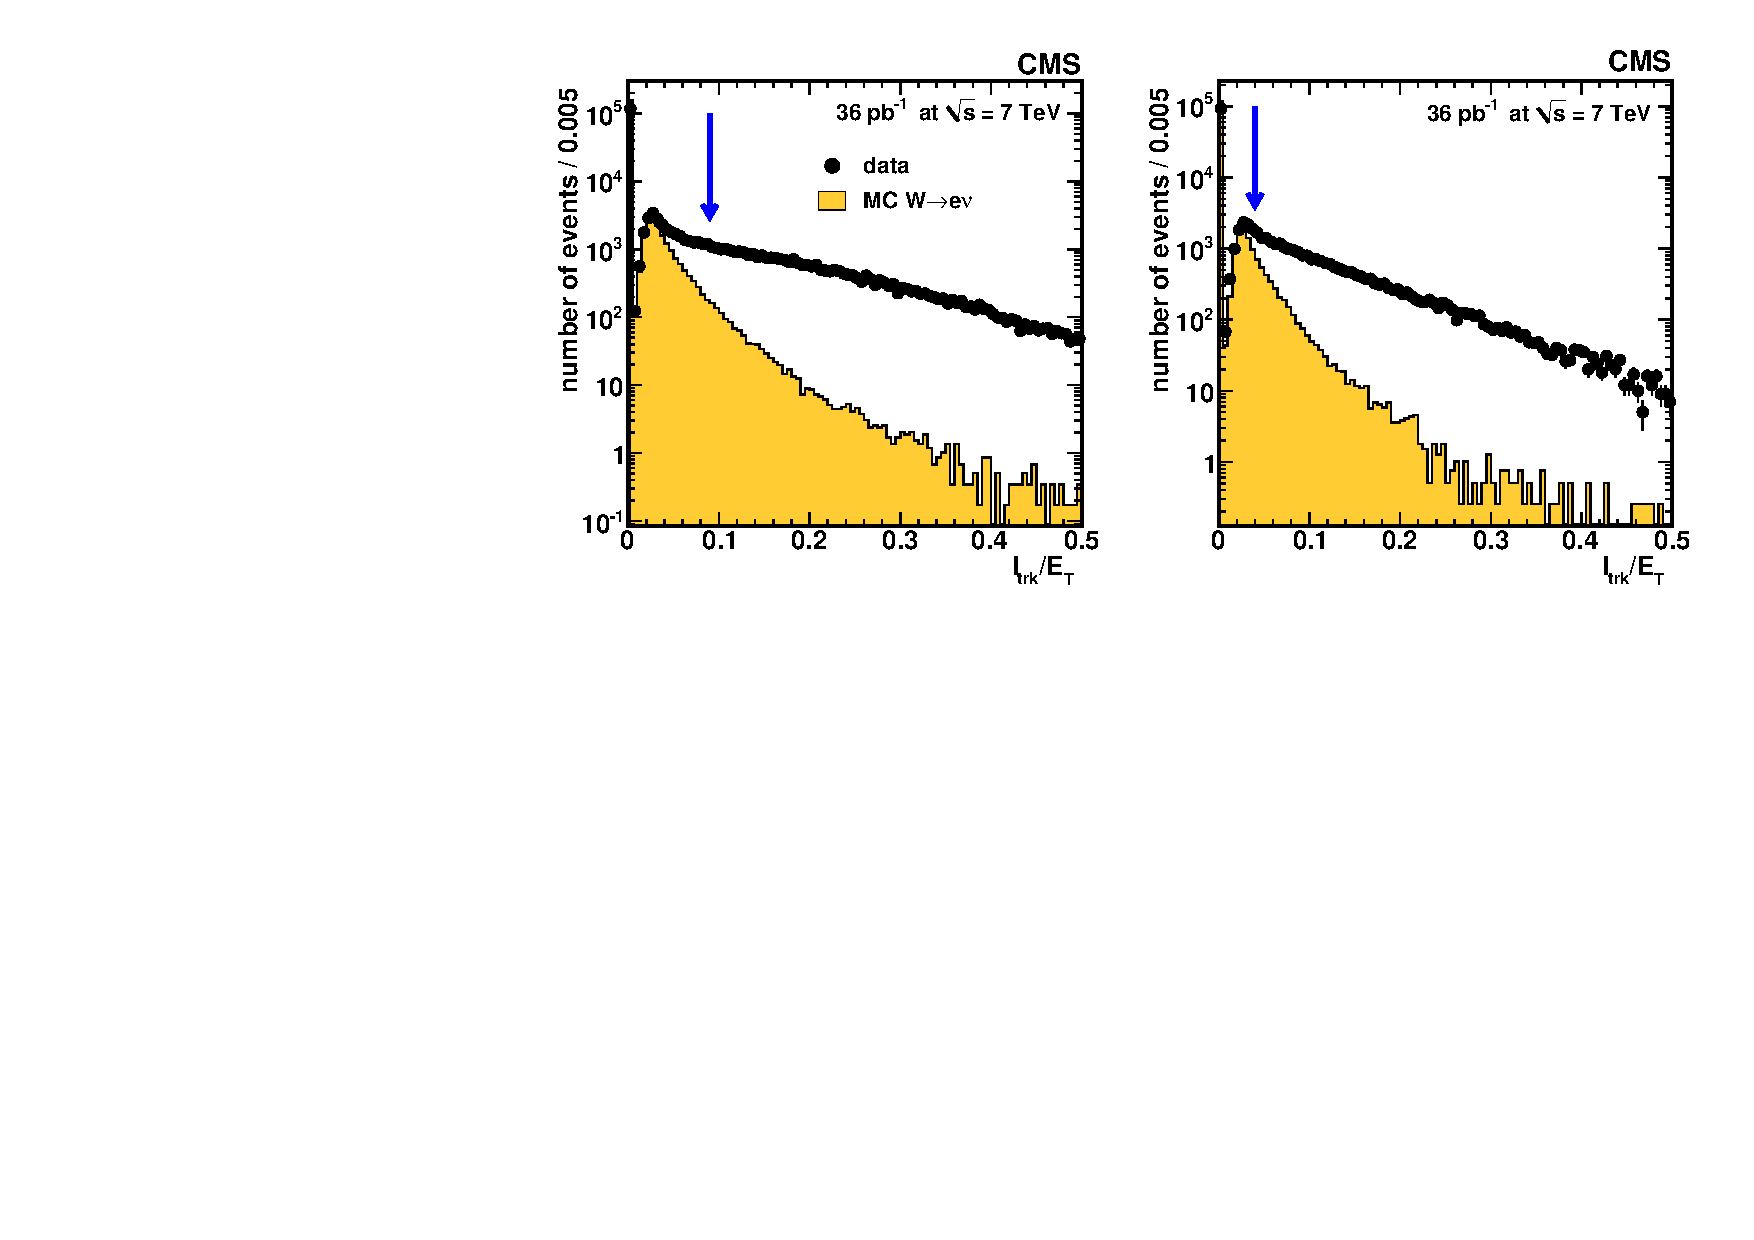
\includegraphics[width=0.68\textwidth]{figs/tkiso.pdf}
   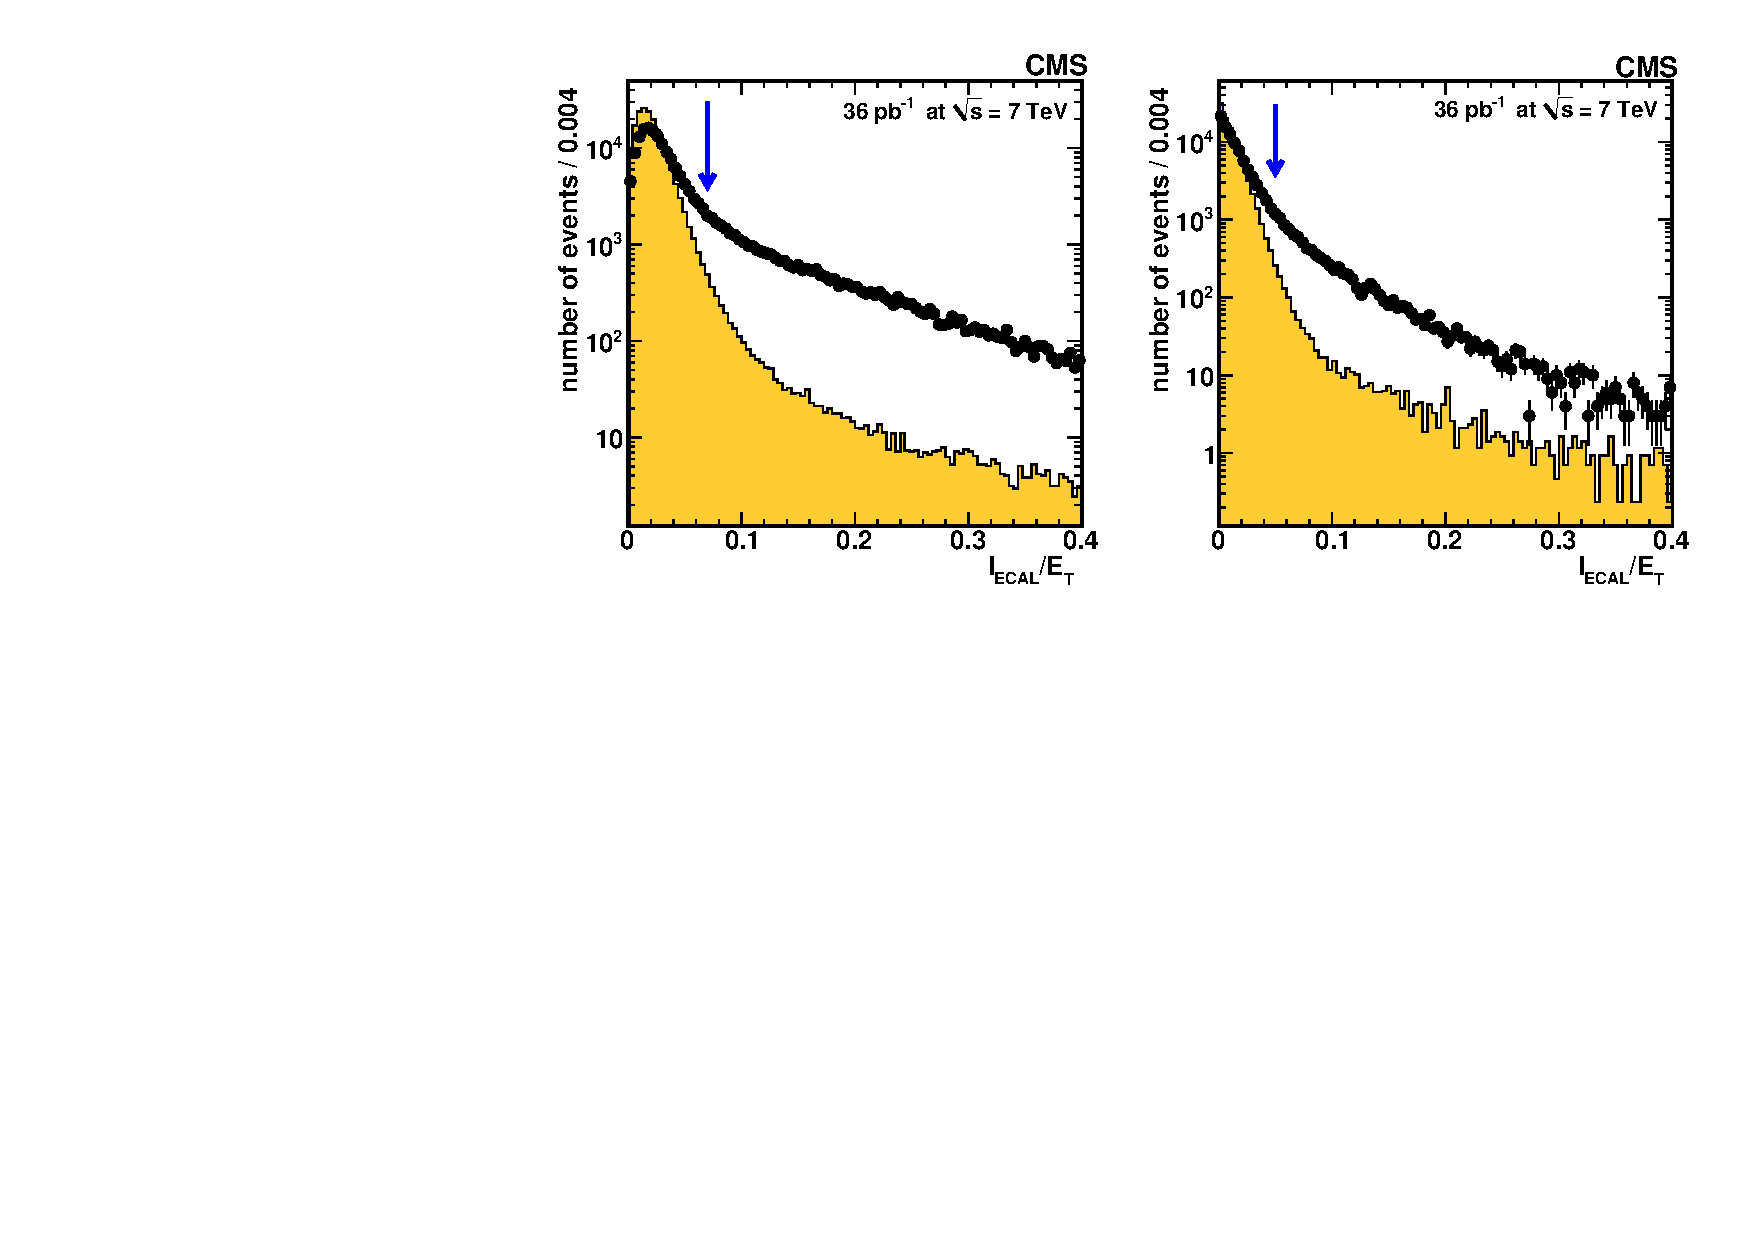
\includegraphics[width=0.68\textwidth]{figs/ecaliso.pdf}
   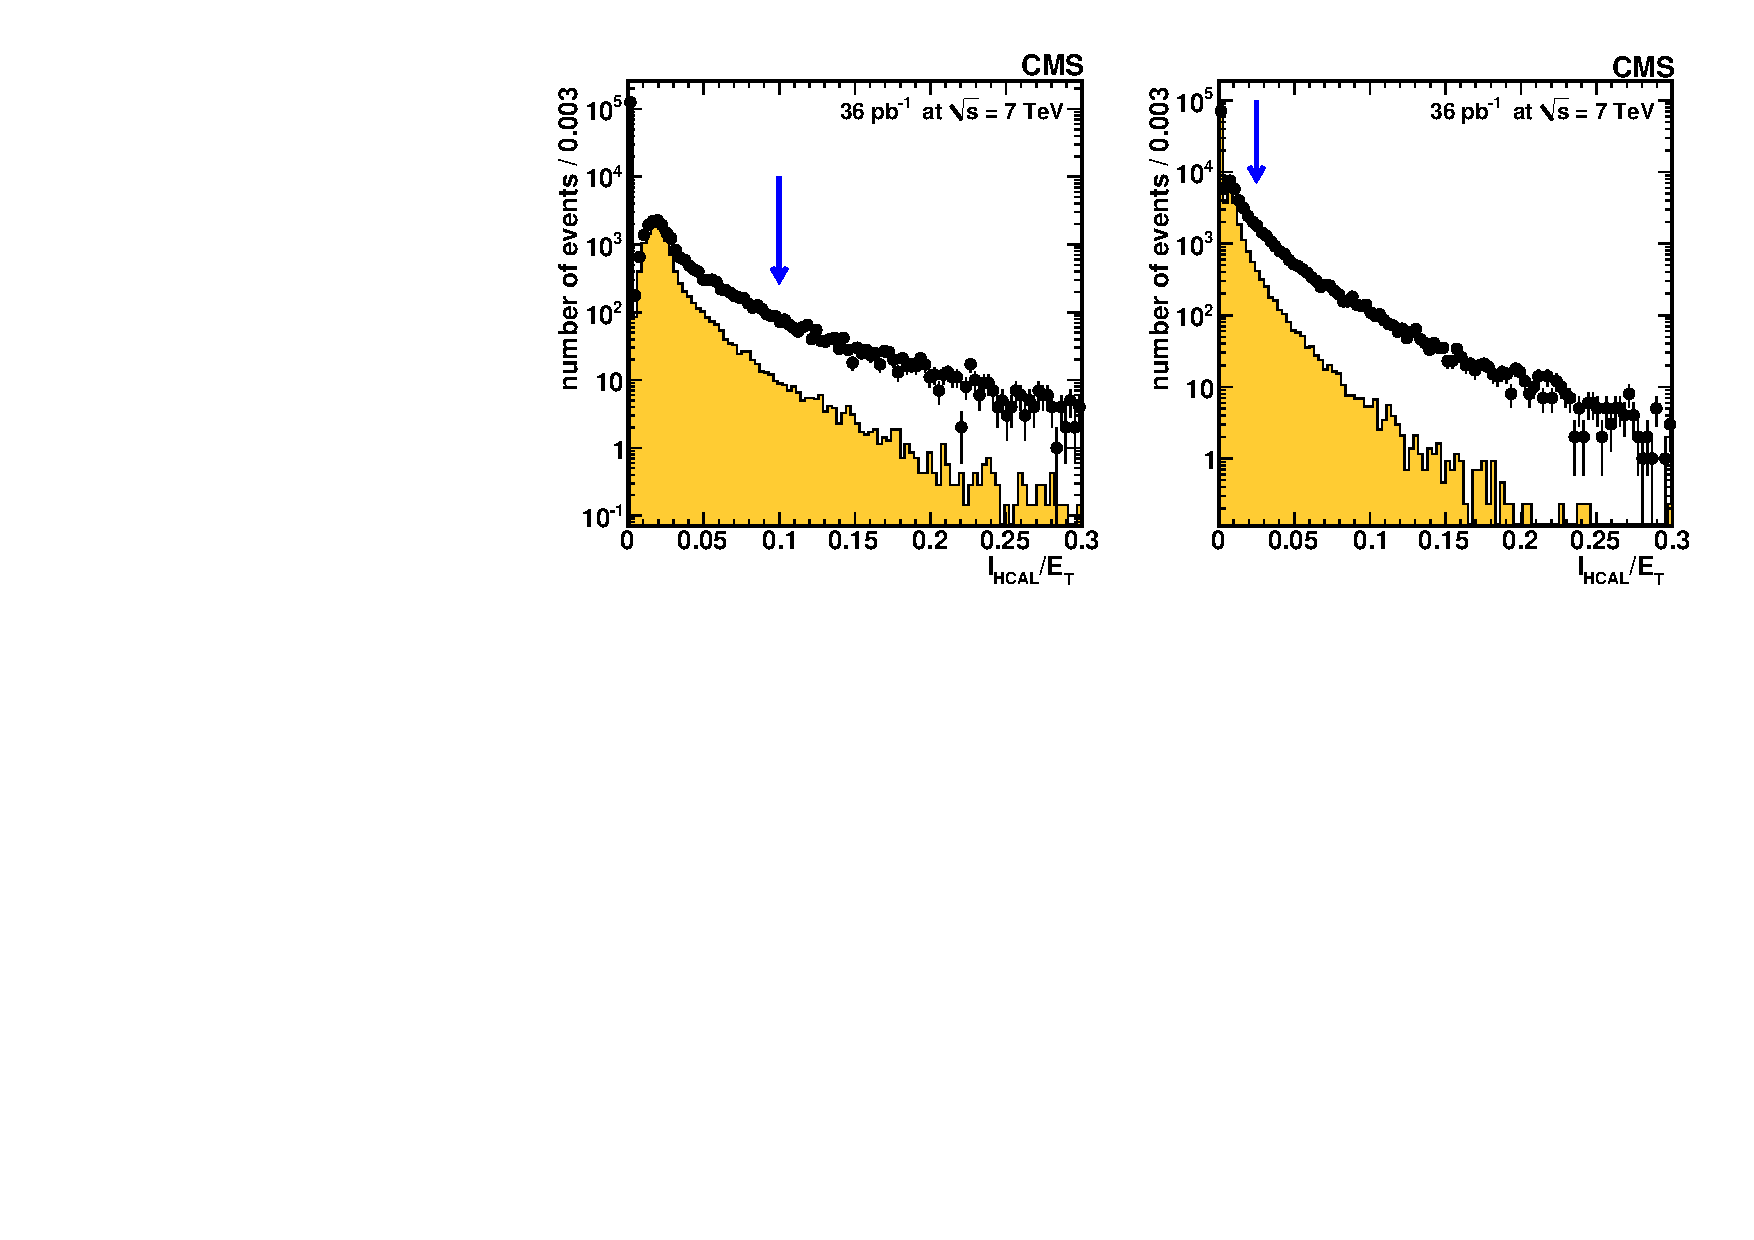
\includegraphics[width=0.68\textwidth]{figs/hcaliso.pdf}
   \caption{ \label{fig:WenuSelection2}
Distributions of the electron isolation variables $\ITRK/\Et$, $\IECAL/\Et$, and $\IHCAL/\Et$
for data (points with the error bars), for EB (left) and EE (right).
For illustration the simulated $\Wen$ signal (histograms), normalized to the number of events
observed in data, is superimposed.
These distributions are obtained after applying all
the tight requirements on the selection variables, except that on the presented
variable. The tight requirement on that variable is indicated with an arrow. }
  \end{center}
\end{figure}
%%%%%

The radiated photons may convert close to the
original electron trajectory, leading to charge misidentification.
Three different methods are used to determine the electron charge. First, the electron 
charge is determined by the signed curvature of the associated GSF track. Second, the charge 
is determined from the associated trajectory reconstructed in the silicon tracker using a 
Kalman Filter algorithm~\cite{KF}. Third, the electron charge is determined based on the azimuthal 
angle between the vector joining the nominal interaction point and the ECAL cluster 
position and the vector joining the nominal interaction point and innermost hit of the GSF track. 
The electron charge is determined from the two out of three charge estimates that are in agreement.
The electron charge misidentification rate is measured in data using the $\Zee$ data
sample to be within 0.1$\%$--1.3$\%$ in EB and 1.4$\%$--2.1$\%$ in EE, increasing with
electron pseudorapidity.


Events are selected if they contain one or two electrons having $\Et>25~\gev$ 
for the $\Wen$ or the $\Zee$ analysis, respectively. 
For the  $\Zee$ selection there is no requirement on the charges of the electrons.
The energy of an electron candidate with $\Et>25~\gev$ is 
determined by the ECAL cluster energy, while its momentum direction is determined by 
that of the associated track. 

Particles misidentified as electrons are suppressed by requiring that the $\eta$ and $\phi$ coordinates
of the track trajectory extrapolated to the ECAL match those
of the ECAL cluster permitting only small differences ($\Delta\eta$, $\Delta\phi$) 
between the coordinates, by requiring a narrow ECAL cluster width in $\eta$ ($\sigma_{\eta\eta}$), 
and by limiting the ratio of the hadronic energy $H$ to the electromagnetic 
energy $E$ measured in a cone of $\Delta R = 0.15$ around the ECAL cluster direction.
More details on the electron identification variables can be found in Refs.~\cite{EGMid,PhotonQCD}. 
Electron isolation is based on requirements on the three isolation 
variables $\IHCAL/\Et$, $\IECAL/\Et$, and $\ITRK/\Et$.

\par
Electrons from photon conversions are suppressed by requiring the 
reconstructed electron track to have at least one hit in the innermost pixel layer.
Furthermore, electrons are
rejected when a partner track is found that is consistent with a
photon conversion, based on the opening angle and the separation in
the transverse plane at the point where the electron and partner
tracks are parallel.

The electron selection criteria were obtained
by optimizing signal and background levels according to
simulation-based studies. The optimization was done for EB
and EE separately.  

Two sets of electron selection criteria are considered: 
a tight one and a loose one.
Their efficiencies, from simulation studies based on $\Wen$ events, are
approximately 80$\%$ and 95$\%$, respectively. These efficiencies correspond 
to reconstructed electrons within the geometrical and kinematic 
acceptance, which is defined in Section~\ref{sec:acceptance}.  
The tight selection criteria give a purer sample of prompt 
electrons and are used for both the $\Wen$ and $\Zee$ analyses.
The virtue of this choice is to have consistent electron definitions 
for both analyses, simplifying the treatment of systematic 
uncertainties in the $\mathrm{W}/\mathrm{Z}$ ratio measurement. 
In addition, the tight working point, applied to both electrons
in the $\Zee$ analysis, reduces the QCD backgrounds to a negligible level.
%%The values of the cuts for the tight and "loose" selection sets are 
%%listed in Table~\ref{tab:electron_cuts}.
%%%%% GD
Distributions of the selection variables are shown in Figs.~\ref{fig:WenuSelection1}
and~\ref{fig:WenuSelection2}.
The plots show the distribution of data together with the simulated signal 
normalized to the same number of events as the data, after applying all 
the tight requirements on the selection variables except the requirement on the displayed
variable. 
%The tight cut on that variable is shown with a vertical line.



For the W analysis, an event is also rejected if there is a second electron 
that passes the loose selection with $\Et > 20~\gev$. This requirement reduces
the contamination from DY events.  
The number of $\Wen$ candidate events selected in the data sample is 
$\WEISAMPLE$, with $\WEPSAMPLE$ positrons and $\WEMSAMPLE$ electrons.

For the Z analysis, two electrons are required within the ECAL acceptance, 
both with $\Et > 25~\gev$ and both satisfying the tight electron selection. 
Events in the dielectron mass region of $60 < m_{\mathrm{ee}} < 120$~GeV are counted.
These requirements select $\ZEESAMPLE$ events.



% \begin{table}[htb]
% \caption{Selection cuts for electrons.}
% \label{tab:electron_cuts}
% \begin{center}
% \begin{tabular}{ | l || c | c || c | c |}
% \hline
%           & \multicolumn{2}{| c ||}{"Loose" e} & \multicolumn{2}{| c |}{tight e} \\
% \hline
%                          & Barrel & Endcap & Barrel & Endcap \\
% \hline \hline
%    $\ITRK/\Et$             & 0.15   & 0.08   & 0.09   & 0.04   \\
% \hline
%    $\IECAL/\Et$              & 2.0    & 0.06   & 0.07   & 0.05   \\
% \hline
%    $\IHCAL/\Et$              & 0.12   & 0.05   & 0.10   & 0.025  \\
% \hline
%    Missing hits $\leq$    & 1      & 1      & 0      & 0      \\
% \hline
%    Dcot                  & $-$    & $-$    & 0.02   & 0.02   \\
% \hline
%    Dist                  & $-$    & $-$    & 0.02   & 0.02   \\
% \hline
%    $\sigma_{\eta\eta}$   & 0.01   & 0.03   & 0.01   & 0.03   \\
% \hline
%    \DP                    & $-$    & $-$    & 0.06   & 0.03   \\
% \hline
%    \DE                    & 0.007  & 0.01   & 0.004  & 0.007  \\
% \hline
%    $H/E$                  & 0.15   & 0.07   & 0.04   & 0.025  \\
% \hline
% \end{tabular}
% \end{center}
% \end{table}





